\documentclass[11pt]{article}
\usepackage[margin=1in]{geometry}
\usepackage{amsmath, amssymb, amsthm, esint}
\usepackage{fancyhdr}
\usepackage{tikz, tikz-3dplot}
% \usepackage{hyperref}
\usepackage{enumitem}
\usepackage{float}
\usepackage{booktabs}
\usepackage{array}
\usepackage{cancel}

\setlength{\headheight}{14pt}
\fancyhf{}
\lhead{Discrete Mathematics}
\cfoot{\thepage}

\begin{document}
\pagestyle{plain}
\begin{center}
    \tableofcontents
\end{center}
\newpage
\setcounter{page}{1}
\pagestyle{fancy}
\section{Logic and Proofs}
\subsection{Propositional Logic}
Proposition is a statement that is \textbf{either} true or false, but not both at the same time. We usually represent it with variables like $p$, $q$, and $r$.\\
e.g. "The sky is blue." is a proposition, but "Listen to me" is not. 
\subsubsection{Logical Connectives}
\begin{itemize}
    \item Negation: $\lnot \,p$. It is not the case that $p$.
    \item Conjunction: $p \land q$. "and"
    \item Disjunction: $p \lor q$. "or"
    \item Implication: $p \rightarrow q$. If $p$ then $q$, $q$ if $p$, $q$ is a consequence of $p$, $p$ only if $q$
    \item biconditional: $p \leftrightarrow q$. $(p\rightarrow q)\land(q \rightarrow p)$, $p$ if and only if $q$
\end{itemize}
\subsubsection{Variations of Conditionals}
\begin{itemize}
    \item Implication: $p \rightarrow q$
    \item Converse: $q \rightarrow p$
    \item Inverse: $\lnot p \rightarrow \lnot q$
    \item Contrapositive: $\lnot q\rightarrow \lnot p$. This is logically equivalent to Implication
\end{itemize}
\subsubsection*{Truth Table}
\begin{table}[H]
    \centering
    \hfill
    \begin{minipage}{.32\textwidth}
        \centering
        \begin{tabular}{c|c|c}
            $p$ & $q$ & $p \lor q$\\
            \hline
            T & T & T\\
            T & F & T\\
            F & T & T\\
            F & F & F
        \end{tabular}
    \end{minipage}
    \hfill
    \begin{minipage}{.32\textwidth}
        \centering
        \begin{tabular}{c|c|c}
            $p$ & $q$ & $p \land q$\\
            \hline
            T & T & T\\
            T & F & F\\
            F & T & F\\
            F & F & F
        \end{tabular}
    \end{minipage}
    \hfill
    \begin{minipage}{.32\textwidth}
        \centering
        \begin{tabular}{c|c|c}
            $p$ & $q$ & $p \rightarrow q$\\
            \hline
            T & T & T\\
            T & F & F\\
            F & T & T\\
            F & F & T
        \end{tabular}
    \end{minipage}
    \hfill
\end{table}
\subsubsection*{Example}
Find the truth value of $\boldsymbol{(p \lor q)\rightarrow \lnot \,r}$
\begin{table}[H]
    \centering
    \begin{tabular}{c|c|c|c|c|c}
        $p$ & $q$ & $r$ & $p \lor q$ & $\lnot \,r$& $(p \lor q)\rightarrow \lnot\, r$ \\
        \hline
        T & T & T & T & F & F\\
        T & T & F & T & T & T\\
        T & F & T & T & F & F\\
        T & F & F & T & T & T\\
        F & T & T & T & F & F\\
        F & T & F & T & T & T\\
        F & F & T & F & F & T\\
        F & F & F & F & T & T
    \end{tabular}
\end{table}
\subsection{Application of Propositional Logic}
\subsubsection{Classification of Proposition}
\begin{itemize}
    \item Tautology: Always true. e.g. $p\lor \lnot\,p$
    \item Contradiction: Always false. e.g. $p\land \lnot\,p$
    \item Contingency: Depends on variable. e.g. $p\rightarrow q$
\end{itemize}
\subsubsection{Logical Equivalence $p \equiv q$}
Two statements are logically equivalent if they always have the same truth value in every possible scenario.\\
e.g. $p$ and $q$ are biconditional, i.e. $p \leftrightarrow q$, means that $p$ and $q$ are logically equivalent.
\subsubsection{Laws of Logical Equivalence}
\begin{table}[H]
    \centering
    \renewcommand{\arraystretch}{1.3}
    \begin{tabular}{>{$}l<{$}|l}
        \text{Equivalence} & \text{Name} \\
        \hline
        p \land T \equiv p & Identity laws \\
        p \lor F \equiv p & \\
        \hline
        p \lor T \equiv T & Domination laws \\
        p \land F \equiv F & \\
        \hline
        p \lor p \equiv p & Idempotent laws \\
        p \land p \equiv p & \\
        \hline
        \lnot(\lnot p) \equiv p & Double negation law \\
        \hline
        p \lor q \equiv q \lor p & Commutative laws \\
        p \land q \equiv q \land p & \\
        \hline
        (p \lor q) \lor r \equiv p \lor (q \lor r) & Associative laws \\
        (p \land q) \land r \equiv p \land (q \land r) & \\
        \hline
        p \lor (q \land r) \equiv (p \lor q) \land (p \lor r) & Distributive laws \\
        p \land (q \lor r) \equiv (p \land q) \lor (p \land r) & \\
        \hline
        \lnot(p \land q) \equiv \lnot p \lor \lnot q & De Morgan's laws \\
        \lnot(p \lor q) \equiv \lnot p \land \lnot q & \\
        \hline
        p \lor (p \land q) \equiv p & Absorption laws \\
        p \land (p \lor q) \equiv p & \\
        \hline
        p \lor \lnot p \equiv T & Negation laws \\
        p \land \lnot p \equiv F & \\
        \hline
        p \rightarrow q \equiv \lnot p \lor q & Conditional\\
        p \rightarrow q \equiv \lnot q \rightarrow \lnot p & \\
        \hline
        p \leftrightarrow q \equiv (p \rightarrow q) \land (q \rightarrow p) & Biconditional\\
        p \leftrightarrow q \equiv \lnot p \leftrightarrow \lnot q & \\
    \end{tabular}
\end{table}
\subsubsection{Determine Logical Equivalence: }
\begin{enumerate}
    \item Verify with Truth Table
    \item Apply Known knowledge
\end{enumerate}
\subsubsection*{Show that $p\rightarrow q$ is logically equivalent to $\lnot q \rightarrow \lnot p$}
\begin{table}[H]
    \centering
    \begin{tabular}{c|c|c|c}
        $p$ & $q$ & $p \rightarrow q$ & $\lnot q\rightarrow \lnot p$ \\
        \hline
        T & T & T & T\\
        T & F & F & F\\
        F & T & T & T\\
        F & F & T & T\\
    \end{tabular}
\end{table}
\subsubsection*{Show that $(p\rightarrow r)\lor (q\rightarrow r) \equiv (p\land q)\rightarrow r$}
\begin{align*}
    (p\rightarrow r)\lor (q\rightarrow r) &\equiv(\lnot p \lor r)\lor (\lnot q \lor r)\\
    &\equiv(\lnot p \lor \lnot q)\lor(r\lor r)\\
    &\equiv\lnot(p\land q) \lor r\\
    &\equiv (p\land q)\rightarrow r _\#
\end{align*}
\subsection{Predicate and Quantifier}
\subsubsection{Predicate}
A predicate is a statement with variables that becomes true or false only once specific values are substituted. $P(x)$ denotes a predicate involving $x$.\\
e.g. Let $P(x)$ be the statement "x>4." We read $P(x)$ as "$x$ is greater than $4$."
\begin{itemize}
    \item $P(x)$ is true if x = 5
    \item $P(x)$ is false if x = 3
\end{itemize}
\subsubsection*{General Form}    
$P(x_1, x_2, x_3, \dots, x_n)$ where each $x_i$ is a variable from the domain of discourse. 
\subsubsection{Quantifier}
\begin{itemize}
    \item Universal quantifier $\forall$: "for all", "every".
    \item Existential quantifier $\exists$: "there exists", "some", "at least one".
\end{itemize}
\subsubsection*{Rules for Quantifier}
Negation of quantifier
\[
    \begin{cases}
        \lnot \forall x \,P(x) \equiv \exists x \,\lnot P(x)\\
        \lnot \exists x \,P(x) \equiv \forall x\, \lnot P(x)
    \end{cases}
\]
Nested quantifier
\[
    \forall x \,\exists y \,P(x, y) \neq \exists y \,\forall x \,P(x, y)
\]
Negation of nested quantifier
\[
    \begin{split}
        \lnot \left(\forall x\, \exists y \, P(x, y)\right) \equiv \exists x\, \forall y\, \lnot P(x, y)\\[.5em]
        \lnot \left(\exists x\, \forall y \, P(x, y)\right) \equiv \forall x\, \exists y\, \lnot P(x, y)
    \end{split}
\]
\subsection{Rule of Inference}
An \textbf{argument} is an implication of the form:
\[
    \bigwedge_{i\in D} p_i \rightarrow q
\]
where $D$ is domain of discourse, $p_i$ is a premise, and $q$ is a conclusion\\
\textbf{Notation:}
\[
    (p \rightarrow q) \land p \quad\therefore q \quad\Rightarrow\quad
    \begin{array}{ll}
        & p \to q \\
        \land & p \\
        \hline \therefore & \multicolumn{1}{c}{q}
    \end{array}
    \quad\Rightarrow\quad
    \begin{array}{l}
        p \to q \\
        p \\
        \hline
        \multicolumn{1}{c}{\therefore \,q}
    \end{array}
\]
\begin{table}[H]
    \centering
    \renewcommand{\arraystretch}{1.3}
    \begin{tabular}{l | >{$}c<{$} | l | >{$}c<{$}}
        \text{Name} & \text{Expression} & \text{Name} & \text{Expression} \\
        \hline
        Modus Ponens & 
        \begin{array}{l}
            p \to q \\
            p \\
            \hline
            \multicolumn{1}{c}{\therefore \,q}
        \end{array} &
        Modus Tollens & 
        \begin{array}{l}
            p \to q \\
            \lnot q \\
            \hline
            \multicolumn{1}{c}{\therefore \,\lnot p}
        \end{array} \\
        \hline
        Hypothetical Syllogism & 
        \begin{array}{r}
            p \to q \\
            q \to r \\
            \hline
            \multicolumn{1}{l}{\therefore p\to r}
        \end{array} &
        Conjunction & 
        \begin{array}{l}
            p\\
            q\\
            \hline
            \therefore \,p\,_\land\,q
        \end{array} \\
        \hline
        Disjunctive Syllogism & 
        \begin{array}{l}
            p \,_\lor\, q\\
            \lnot p\\
            \hline
            \multicolumn{1}{c}{\therefore \,q}
        \end{array} &
        Addition & 
        \begin{array}{c}
            p\\
            \hline
            \multicolumn{1}{c}{\therefore p\,_\lor\,q}
        \end{array} \\
        \hline
        Simplification & 
        \begin{array}{c}
            p \,_\land\, q\\
            \hline
            \therefore\, p\\
            \therefore\, q
        \end{array} &
        Resolution & 
        \begin{array}{r}
            p \,_\lor\, q\\
            \lnot p \,_\lor\, r\\
            \hline
            \multicolumn{1}{c}{\therefore q\,_\lor\,r}
        \end{array} \\
    \end{tabular}
\end{table}
\subsubsection*{Rules for Quantified Statement}
\textbf{Universal Instantiation:} From a universal statement $\forall x\, P(x)$, we may infer $P(c)$ for any particular $c$.  
\[
    \forall x\, P(x) \;\;\Rightarrow\;\; P(a)
\]
\textbf{Universal Generalization:} If $P(c)$ holds for an arbitrary element $c$, then we may conclude $\forall x\, P(x)$.  
\[
    P(c) \;\;\Rightarrow\;\; \forall x\, P(x)
\]
\textbf{Existential Instantiation:} From $\exists x\, P(x)$, we may introduce a new symbol $c$ such that $P(c)$ holds.  
\[
    \exists x\, P(x) \;\;\Rightarrow\;\; P(c)
\]
\textbf{Existential Generalization:}   From $P(c)$ for a particular $c$, we may conclude $\exists x\, P(x)$.  
\[
    P(c) \;\;\Rightarrow\;\; \exists x\, P(x)
\]
\subsection{Introduction to Proofs}
\subsubsection{Some Mathematical Terminology}
\begin{itemize}
    \item \textbf{Theorem:} A major, important mathematical statement that has been proved true.
    \item \textbf{Lemma:} A proved result used mainly as a stepping stone toward a larger theorem.
    \item \textbf{Corollary:} A statement that follows directly and easily from a theorem or proposition.
    \item \textbf{Proposition:} A proved statement that is true but of smaller or less central importance than a theorem.
    \item \textbf{Conjecture:} A mathematical claim believed to be true but not yet proved.
    \item \textbf{Proof:} A logical argument that establishes the truth of a mathematical statement beyond doubt.
\end{itemize}
\subsubsection{Types of Proof}
\begin{itemize}
    \item\textbf{Direct Proof:}
        Show a statement is true by straightforward logical reasoning from definitions and known results.\\[.5em]
        \textbf{Example:} Prove that if $n$ is odd, then $5n+3$ is even.\\
        \textit{Proof:}\\
        Let $n = 2k + 1, k \in \mathbb{Z}$, then 
        \[
            5n+3 = 2(2k+1)+3=10n+8=2(5k+4)
        \]So, $5n+3=2(5k+4)$ and $5k+4\in\mathbb{Z}$\[\therefore 5n+3\text{ is even}_\#\]
    \item\textbf{Proof by Contrapositive:}
        Show a statement is true by proving that if the conclusion is false, then the premise must also be false.\\[.5em]
        \textbf{Example:} Prove that if $n$ is odd, then $5n+3$ is even.\\
        \textit{Proof:}
    \item\textbf{Proof by Contradiction:}
        Show a statement is true by assuming the opposite and deriving a contradiction.\\[.5em]
        \textbf{Example:} Prove that $\sqrt{2}$ is irrational\\
        \textit{Proof:}\\
        Let \begin{align*}
            &\sqrt{2} = \frac{p}{q},\;q\neq 0,\;p,q\in\mathbb{N},\;\gcd(p,q)=1\\
            &\Rightarrow 2 = \frac{p^2}{q^2} \Rightarrow 2q^2 = p^2
        \end{align*}
        Thus, $2\,|\,p^2$, so $2\,|\,p$. We have
        \[
            p=2k,\;k\in\mathbb{N}, \;4k^2 = 2q^2 \Rightarrow 2k^2 = q^2
        \]
        Similarly, $2\,|\,q$. Concluding 
        \[
            2\,|\,\gcd(p,q) \Rightarrow\!\Leftarrow
        \]
        Thus $\sqrt{2}$ is irrational. 
    \item\textbf{Proof by Cases:}
        Show a statement is true by dividing into cases and proving it holds in each case.\\[.5em]
        \textbf{Example:}\\
        \textit{Proof:}\\
    \item\textbf{Methametical Induction:}
        Show a statement is true by proving a base case and then proving the inductive step from n to n+1.\\[.5em]
        \textbf{Example:}\\
        \textit{Proof:}\\
    \item\textbf{Existence and Uniqueness Proof}
        Show a statement is true by first proving that at least one object with the required property exists (existence), and then proving that no more than one such object can exist (uniqueness).\\[.5em]
        \textbf{Example:} Prove that if $\displaystyle r \in \mathbb{Q}^{\,c}$, then $\displaystyle\exists !\, n \in \mathbb{Z} \;|r-n| < \frac{1}{2}$.\\
        \textit{Proof:}\\
        Let 
        \[
            n = \lfloor r + \frac{1}{2} \rfloor
        \]
        By definition we have
        \[
            n \leq r + \frac{1}{2}< n + 1
        \]
        Hence \[|r-n| < \tfrac{1}{2}\], so such an integer $n$ exists. (Existence)\\
        Suppose
        \[
            \exists m,\, m\neq n,\,|r-m|<\frac{1}{2}
        \]
        Consider
        \begin{align*} 
            |n-m| &= |(n-r)+(r-m)|\\
            &\leq|n-r| + |r-m|\\
            &=\frac{1}{2}+\frac{1}{2}=1
        \end{align*}
        Since $n$ and $m$ are integers, the inequality $|n-m| < 1$ implies $n = m$. Therefore, the integer $n$ is unique. (Uniqueness)
\end{itemize}
\section{Sets}
\subsection{Definition and Notation}
A \textbf{set} is a well-defined collection of distinct objects, called \textbf{elements}.  
If $a$ is an element of the set $A$, we write $a \in A$. If $a$ is not an element of $A$, we write $a \notin A$.
Sets are usually denoted by capital letters $A, B, C \dots$
\begin{itemize}
    \item Roster Method: List all of its elements within curly braces $\{a, b, c, \dots\}$
    \item Set-builder Notations: $\{x \mid \text{condition on }x \}$
\end{itemize}
\textbf{Example:} The set of all positive integers less than 100: $\{x\in \mathbb{Z}^+ \mid x < 100\}$
\subsection{Common Sets of Numbers and their Definitions}
\begin{itemize}
    \item $\mathbb{N}$: The set of \textbf{natural numbers}. (Sometimes defined to include $0$.)
    \[
        \mathbb{N} = \{1, 2, 3, \dots\}
    \]
    \item $\mathbb{Z}$: The set of \textbf{integers}. These can be expressed as the difference of two natural numbers.
    \[
        \mathbb{Z} = \{a - b \mid a, b \in \mathbb{N}\}
    \]
    \item $\mathbb{Q}$: The set of \textbf{rational numbers}. These are ratios of two integers with nonzero denominator.
    \[
        \mathbb{Q} = \left\{\frac{a}{b} \;\middle|\; a, b \in \mathbb{Z}, b \neq 0 \right\}
    \]
    \item $\mathbb{R}$: The set of \textbf{real numbers}. Formally constructed as the set of equivalence classes of The limits of infinite convergent Cauchy sequences of rational numbers. That is,
    \[
        \mathbb{R} = \left\{ \lim_{n \to \infty} a(n) \mid a: \mathbb{N}\to\mathbb{Q},\,\forall \epsilon > 0, \exists N \in \mathbb{N},\, \left|a(n) - a(N)\right| < \epsilon\right\}
    \]
    where a sequence $a(n)$ is \emph{Cauchy} if $\forall \, \varepsilon > 0, \exists N \in \mathbb{N}$ such that $\forall m,n > N$, $|a(m) - a(n)| < \varepsilon$.
    \item $\mathbb{C}$: The set of \textbf{complex numbers}. Defined as ordered pairs of real numbers with special addition and multiplication rules
    \[
        \mathbb{C} = \{a + bi \mid a, b \in \mathbb{R}, \; i^2 = -1\}.
    \]
\end{itemize}
\subsection{Subsets, Subsets, Cardinality, and Power Sets}
\textbf{Subsets:} A set $A$ is a subset of $B$ if every element of $A$ is also in $B$.
\[
    A \subseteq B \quad \iff \quad \forall x \ (x \in A \implies x \in B)
\]
\textbf{Proper Subsets:} A set $A$ is a proper subset of $B$ if $A\subseteq B$ and $A \neq B$.
\[
    A \subset B \quad \iff \quad A \subseteq B \ \text{and} \ A \neq B
\]
\textbf{Cardinality:} The number of elements in a set $A$, denoted $|A|$.
\[
    | \{1,2,3\} | = 3, \quad | \varnothing | = 0
\]
\textbf{Power Set:} The set of all subsets of $A$.
\[
    \mathcal{P}(A) = \{ B \mid B \subseteq A \}, \quad |\mathcal{P}(A)| = 2^{|A|}
\]
\subsection{Set Operations}
\begin{itemize}
    \item Union: $A\cup B = \{x \mid x \in A \text{ or } x \in B\}$ 
    \item Intersection: $A\cap B = \{x \mid x \in A \text{ and } x \in B\}$ 
    \item Difference: $A - B \text{ or }A/B = \{x \mid x \in A \text{ and } x \notin B\}$
    \item Complement: $\bar{A} \text{ or } A^c = \{x \in U \mid x \notin A\}$
    \item Cartesian Product of sets $A_i$ is defined by:
        \[
            A_1\times A_2 \times \cdots \times A_n  = \{ (a_1, a_2, \dots, a_n) \mid a_i \in A_i \}
        \]
        if $A_1 = A_2 = \cdots = A_n$, then $A_1\times A_2 \times \cdots \times A_n = A_{1}^n$
    \end{itemize}
\section{Functions}
\subsection{Definition and Notation}
A function $f$ from a set $A$ to $B$, written $f: A\to B$ is a mapping defined by
\[
    a \in A \to f(a) \in B
\]
To check if $f: A\to B$ is a function
\begin{enumerate}
    \item Algebraically: if $a_1 = a_2$, then it follows $f(a_1) = f(a_2)$
    \item Geometrically: Vertical Line Test, i.e., for every vertical line $x = a$, the graph of $f$ interescts the line in at most one point.
\end{enumerate}
\subsection{Domain, Codomain, and Range}
Let $f : A \to B$ be a function.
\begin{itemize}
    \item The set $A$ is called the \textbf{domain} of $f$.
    \item The set $B$ is called the \textbf{codomain} of $f$.
    \item For each $a \in A$, the element $f(a) \in B$ is called the \textbf{image} of $a$ under $f$.
    \item The set 
    \[
        \text{Range}(f) = \{ f(a) \mid a \in A \}
    \]
    is called the \textbf{range} (or image) of $f$.  
    Note that $\text{Range}(f) \subseteq B$, i.e., the range is always a subset of the codomain.
\end{itemize}
\begin{figure}[H]
    \centering
    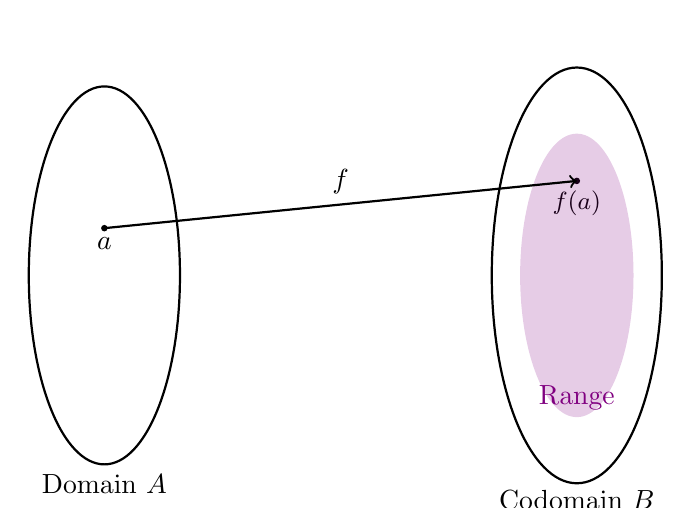
\begin{tikzpicture}[scale=1.2]
        \draw[thick] (0,0) ellipse (0.8 and 2) node[below=2.4cm] {Domain $A$};
        \draw[fill=black] (0, .5) circle (.8pt) node[below] {$a$};

        \draw[thick] (5,0) ellipse (0.9 and 2.2) node[below=2.6cm] {Codomain $B$};
        \draw[fill=black] (5,1) circle (.8pt) node[below] {\small $f(a)$};

        \begin{scope}
            \clip (5,0) ellipse (0.9 and 2.2);
            \fill[opacity=0.2, violet] (5,0) ellipse (0.6 and 1.5);
        \end{scope}
        \node[violet] at (5,-1.3) {Range};

        \draw[->, thick] (0, .5) -- (5, 1) node[midway, above] {$f$};
    \end{tikzpicture}
\end{figure}
\subsection{One-to-one and Onto}
Let $f: A\to B$ be a function. 
\begin{itemize}
    \item f is \textbf{onto (surjective)} if for every $b \in B$, there exists at least one $a$ such that $f(a) = b$.
        \[
            \forall b\in B, \exists a\in A, f(a) = b
        \]
    \item f is \textbf{one-to-one (injective)} if for every $b\in B$, there exists only one $a$ such that $f(a) = b$.
        \[
            \forall a_1, a_2 \in A,\; f(a_1) = f(a_2) \Rightarrow a_1 = a_2
        \]
    \item f is \textbf{bijective} if f is both \textbf{surjective} and \textbf{injective}. Bijection is also called one-to-one correspondenc.
\end{itemize}
\subsection{Sum and Product}
Let $f_1$, $f_2$ be functions $A\to B$. Then $f_1 + f_2$ and $f_1f_2$ are also functions from $A \to B$.\\ Defined for all $x\in A$
\begin{align*}
    &f_1(x) + f_2(x) = (f_1 + f_2)(x)\\
    &f_1(x) \cdot f_2(x) = (f_1 f_2)(x)
\end{align*}
\subsection{Composite and Inverse Function}
\subsubsection{Composite Function}
Let $f: A\to B$ and $g: B \to C$. We denote function composition as $g \circ f: A\to C$, where 
\[
    (g\circ f)(x) = g(f(x))
\]
\begin{figure}[H]
    \centering
    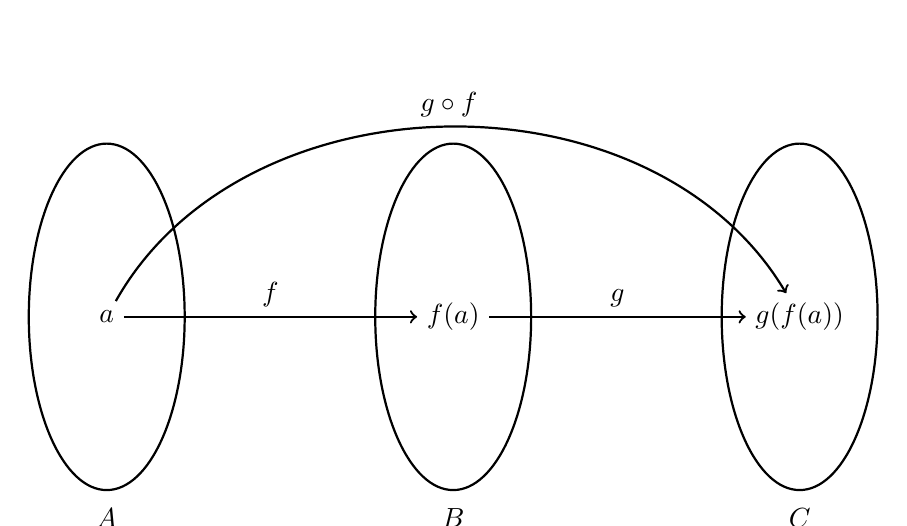
\begin{tikzpicture}[scale=1.1]
        \draw[thick] (0,0) ellipse (0.9 and 2) node[below=2.3cm] {$A$};
        \draw[thick] (4,0) ellipse (0.9 and 2) node[below=2.3cm] {$B$};
        \draw[thick] (8,0) ellipse (0.9 and 2) node[below=2.3cm] {$C$};

        \node at (0,0) (a) {$a$};
        \node at (4,0) (fa) {$f(a)$};
        \node at (8,0) (gfa) {$g(f(a))$};

        \draw[->, thick] (a) -- (fa) node[midway, above] {$f$};
        \draw[->, thick] (fa) -- (gfa) node[midway, above] {$g$};
        \draw[->, thick, bend left=60] (a) to node[midway, above] {$g \circ f$} (gfa);
    \end{tikzpicture}
\end{figure}
\subsubsection{Inverse Functions}
A function $f: A \to B$ has an inverse $f^{-1}: B \to A$ if $f$ is \textbf{bijective}, such that
\[
    f^{-1}(b) = a \iff f(a) = b
\]
Equivalently, two functions $f$ and $g$ are inverses of each other if and only if
\[
    f(g(x)) = g(f(x)) = x
\]
\end{document}